%                             ПРЕАМБУЛАА
\documentclass[a4paper,12pt]{article}
\usepackage[warn]{mathtext}
\usepackage[T1, T2A]{fontenc}
\usepackage[utf8]{inputenc}
\usepackage[russian,english]{babel}
\usepackage{cmap}
\usepackage{amsmath} 
\usepackage{alltt}
\usepackage[left=2cm,right=2cm,top=2cm,bottom=2cm]{geometry}
\usepackage{moreverb}
\usepackage{listings}
\ifx\pdfoutput\undefined
\usepackage{graphicx}
\else
\usepackage[pdftex]{graphicx}
\fi\renewcommand\contentsname{Содержание} 



%-------------------------------------------------------------------------------------------------------------------------------------------------

\begin{document}

\selectlanguage{russian}

\begin{titlepage}
\newpage
\begin{center}
\large «Санкт-Петербургский национальный исследовательский университет информационных технологий, механики и оптики»\\ \hrulefill
\end{center}
\vspace{8em}
\begin{center}
\huge Отчёт по лабораторной работе\\ [10pt]
\end{center}
\vspace{2.5em}
\begin{center}
\large <<Лабораторная работа о информатике №7>>\\
\end{center}

\vspace{6em}

\begin{flushleft}
\emph{Выполнил:} студент 1 курса Липинский Илья (Группа: M3109).\\
\vspace{2.5em}
\emph{Приняла:} Ханжина Наталья Евгеньевна \\
\end{flushleft}

\vspace{\fill}

\begin{center}
Санкт-Петербург 2017
\end{center}

\end{titlepage}

%-------------------------------------------------------------------------------------------------------------------------------------------------

\newpage
\begin{center}
Линейные фильтры
\end{center}

\begin{figure}[h]

\begin{minipage}[h]{0.2\linewidth}
\includegraphics[width=1\linewidth]{Pic}
Исходник. 
\end{minipage}
$\mspace{30mu}$
\begin{minipage}[h]{0.2\linewidth}
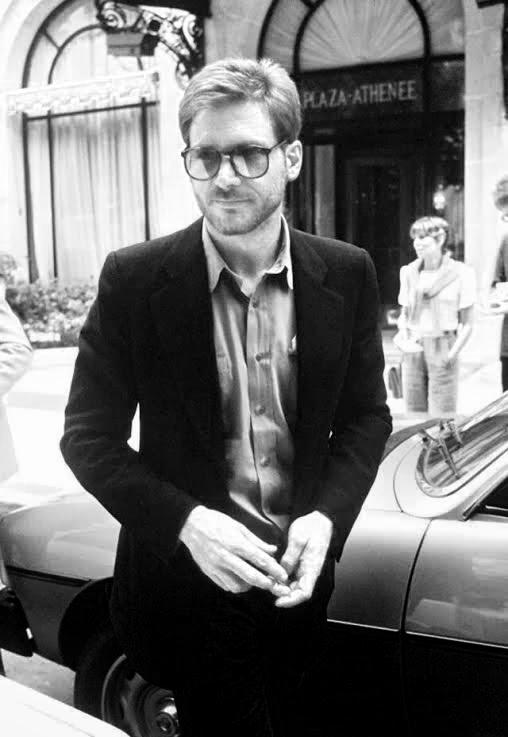
\includegraphics[width=1\linewidth]{Pic_Grey}
Оттенки серого.
\end{minipage}
$\mspace{30mu}$
\begin{minipage}[h]{0.2\linewidth}
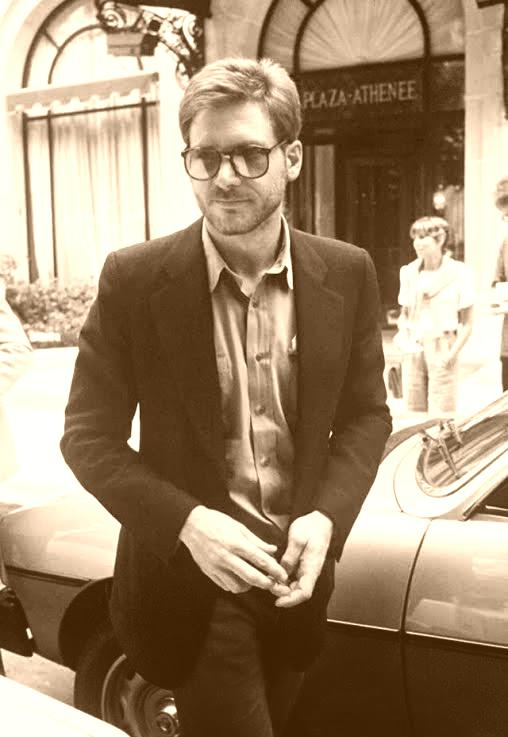
\includegraphics[width=1\linewidth]{Pic_Sepia}
Сепия. 
\end{minipage}
$\mspace{30mu}$
\begin{minipage}[h]{0.2\linewidth}
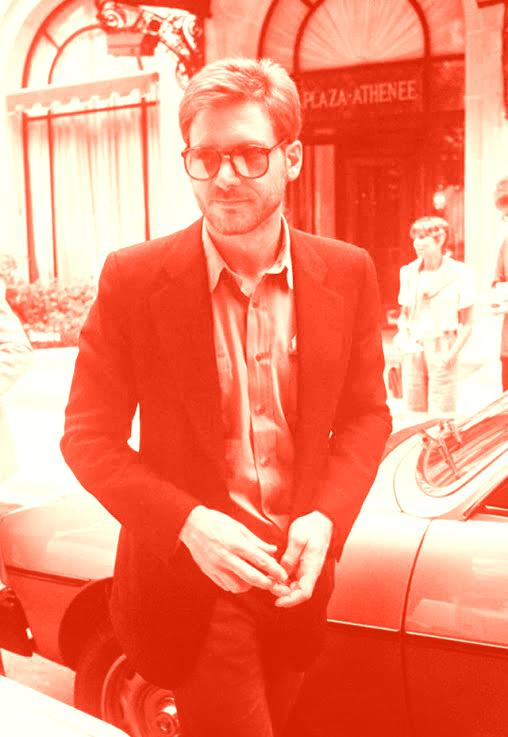
\includegraphics[width=1\linewidth]{Pic_Sepia_red}
Сепия в красном.
\end{minipage}

\vspace{5mm}

\begin{minipage}[h]{0.2\linewidth}
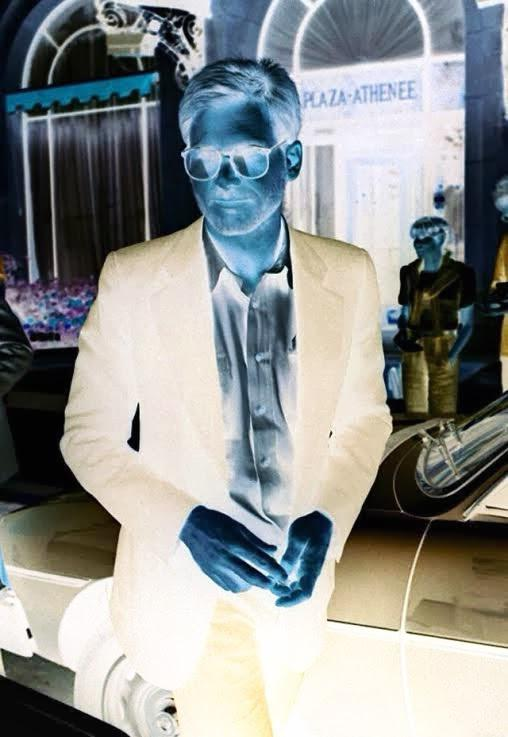
\includegraphics[width=1\linewidth]{Pic_Negative}
Негатив.
\end{minipage}
$\mspace{30mu}$
\begin{minipage}[h]{0.2\linewidth}
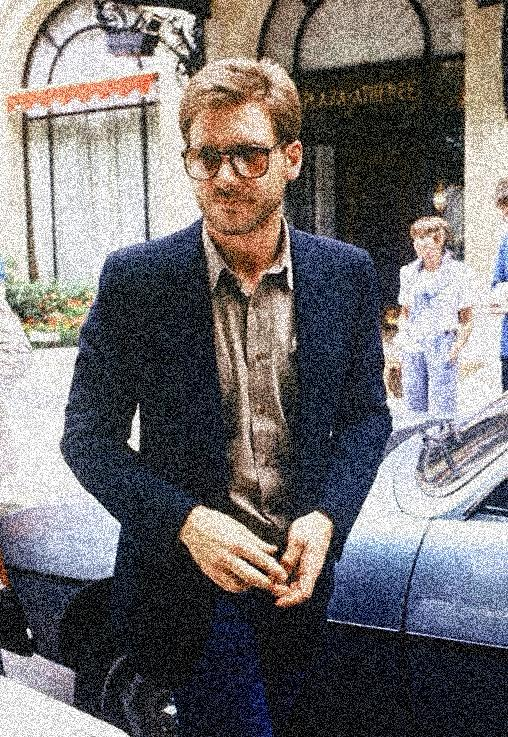
\includegraphics[width=1\linewidth]{Pic_Noises}
Шумы.
\end{minipage}
$\mspace{30mu}$
\begin{minipage}[h]{0.2\linewidth}
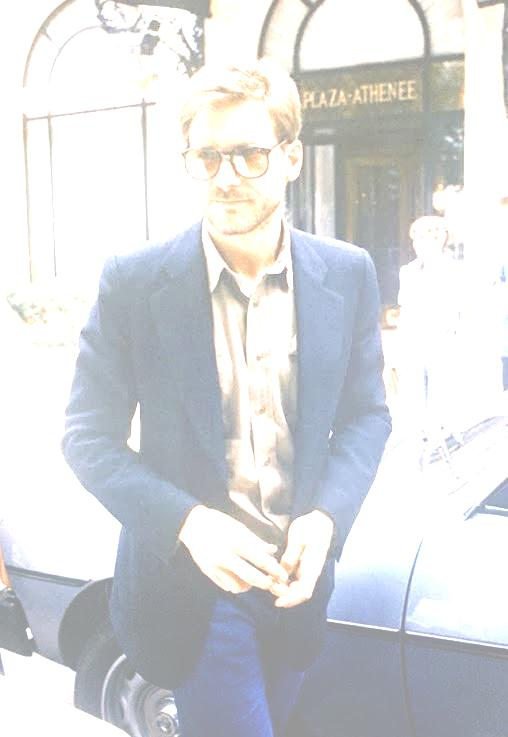
\includegraphics[width=1\linewidth]{Pic_Bright}
Ярче.
\end{minipage}
$\mspace{30mu}$
\begin{minipage}[h]{0.2\linewidth}
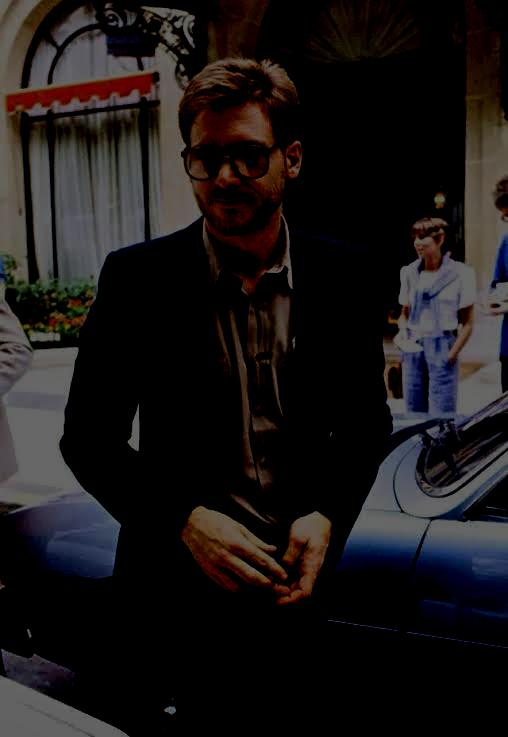
\includegraphics[width=1\linewidth]{Pic_Dark}
Темнее.
\end{minipage}

\vspace{5mm}

\begin{minipage}[h]{0.2\linewidth}
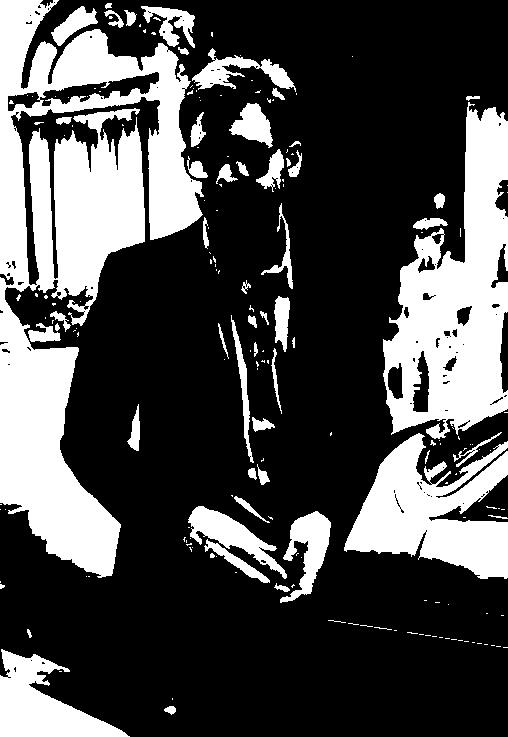
\includegraphics[width=1\linewidth]{Pic_BlackOrWhite}
Только ч/б
\end{minipage}
$\mspace{30mu}$
\begin{minipage}[h]{0.2\linewidth}
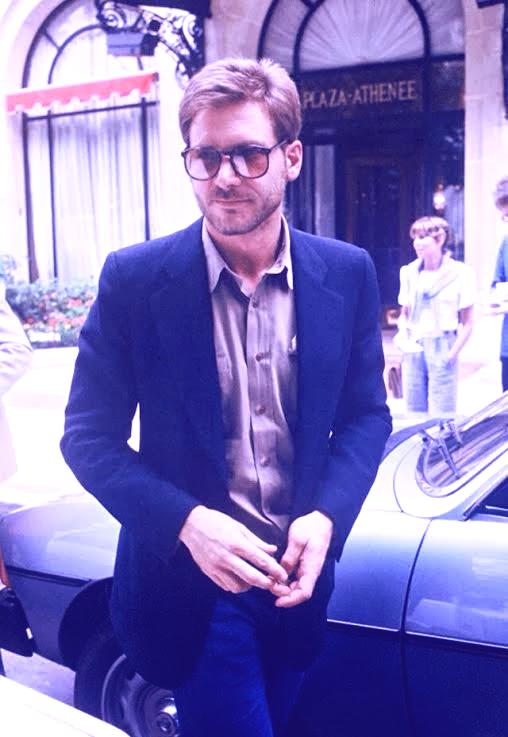
\includegraphics[width=1\linewidth]{Pic_MyFilter}
Мой фильтр.
\end{minipage}

\end{figure}

%-------------------------------------------------------------------------------------------------------------------------------------------------

\newpage
\begin{center}
Матричные фильтры
\end{center}
\vspace{5mm}

\begin{figure}[h]
\begin{center}
\begin{minipage}[h]{0.3\linewidth}
\includegraphics[width=1\linewidth]{Pic}
Исходник. 
\end{minipage}
$\mspace{50mu}$
\begin{minipage}[h]{0.3\linewidth}
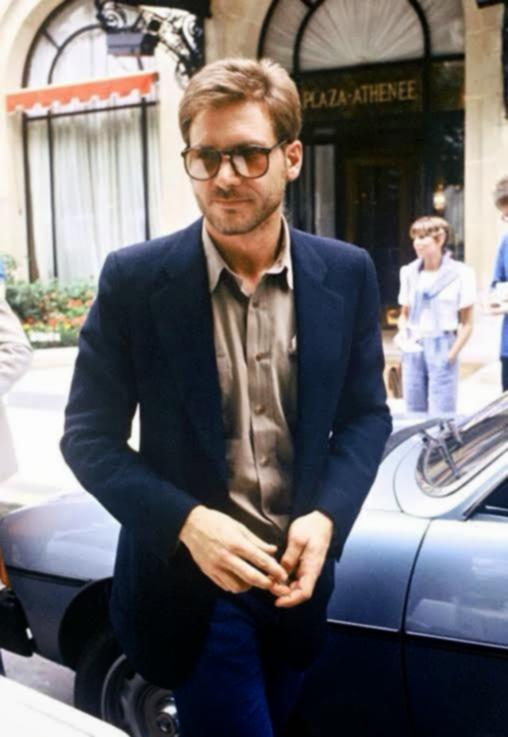
\includegraphics[width=1\linewidth]{Pic_matrix_Gauss_blur}
Размытие. 
\end{minipage}
\end{center}

\vspace{5mm}

\begin{center}
\begin{minipage}[h]{0.3\linewidth}
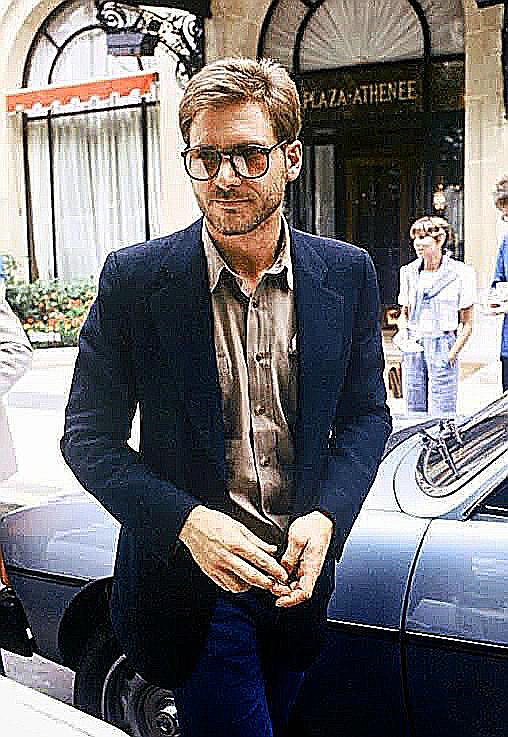
\includegraphics[width=1\linewidth]{Pic_matrix_Sharpness}
Повышенная резкость. 
\end{minipage}
$\mspace{50mu}$
\begin{minipage}[h]{0.3\linewidth}
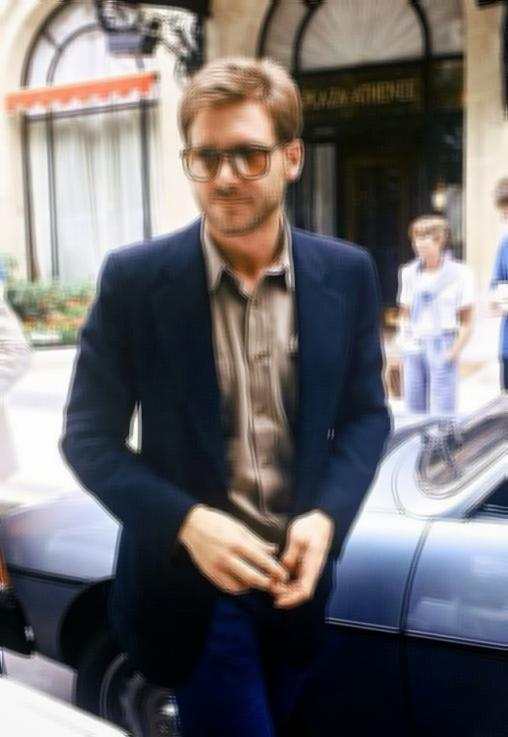
\includegraphics[width=1\linewidth]{Pic_matrix_MyMatrixFilter}
Мой матричный фильтр.
\end{minipage}
\end{center}

\end{figure}

%-------------------------------------------------------------------------------------------------------------------------------------------------

\newpage


\end{document}

